\subsection{Что то про линейную регрессию}
From \eqref{eq:linear_matrix_form} linear model is:
\begin{equation*}
	Y = X \beta
\end{equation*}
$\beta$ - unknown parameters. The residual for this model is:
Now, just substitute the residual to loss function \eqref{eq:loss}:
\begin{equation*}
	\mathcal{L} = \dfrac{1}{N} \sqrt{\sum_{i = 1}^N \left ( R^i \right )^2} \Leftrightarrow \| Y - X \beta \|^2 \rightarrow min
\end{equation*}
\begin{equation}
	\| Y - X \beta \|^2 = \left ( Y - X \beta \right )^T \left ( Y - X \beta \right ) =  Y^T Y - Y^T X \beta - \beta^T X^T Y + \beta^T X^T X \beta
	\label{eq:linear_opt}
\end{equation}
And compute $\dfrac{\partial \mathcal{L}}{\partial \beta}$:
\begin{equation*}
	\dfrac{\partial }{\partial \beta} \left [ Y^T Y - Y^T X \beta - \beta^T X^T Y + \beta^T X^T X \beta \right ] \implies X^T Y =  X^T X \beta \\
	\beta = \left ( X^T X \right )^{-1} X^T Y
\end{equation*}

The last operation was very dangerous in sense when the inverse matrix doesn't exist or ill-conditioned. For example, if the determinant of matrix $X^T X$ doesn't exist what should do? Or $X^T X$ is ill-conditioned?
The answer is to apply the special techniques to avoid it - regularization. 
Look at the \eqref{eq:linear_opt} and add the additional term \cite{kress2012numerical}:
\begin{equation}
	\| Y - X \beta \|^2 + \lambda \| \beta \|^2 \implies \beta = \left ( X^T X + \lambda I \right )^{-1} X^T Y
\end{equation}
From \cite{kress2012numerical} implies fact, that $X^T X + \lambda I$ is not singular matrix and in fact has better condition number than $X^T X$. Moreover, there are a lot of regularization techniques \cite{ridge}, \cite{lasso}, \cite{dantzig_selector}, \cite{rlad}, \cite{slope}. 
It is only one simple example of problems, arises during the approximation process. By the way, more powerful methods exist, avoiding some problems: Random Forest, Gradient Boosting\ cite{bishop}, Neural Networks \cite{haykin}.
\paragraph{Impact of the regularization}
Let $y = f(x) = k  x + \epsilon, k = 10$. At the fig. \ref{fig:regularizations} seen, that regularization impact is big. After applying linear models (\cite{ridge}, \cite{lasso}, \cite{rlad}) for this problem with different regularization methods was got a different results. The RLAD method estimate the $\hat{k} = 10.498$, Ridge method $\hat{k} = 9.109$ and Lasso - $\hat{k} = 9.604$. Results slightly different because the key difference is using different norms for regularization. It is an important fact for the next work, where more complex regression models will be used. 

\begin{figure}[h]
	\centering
	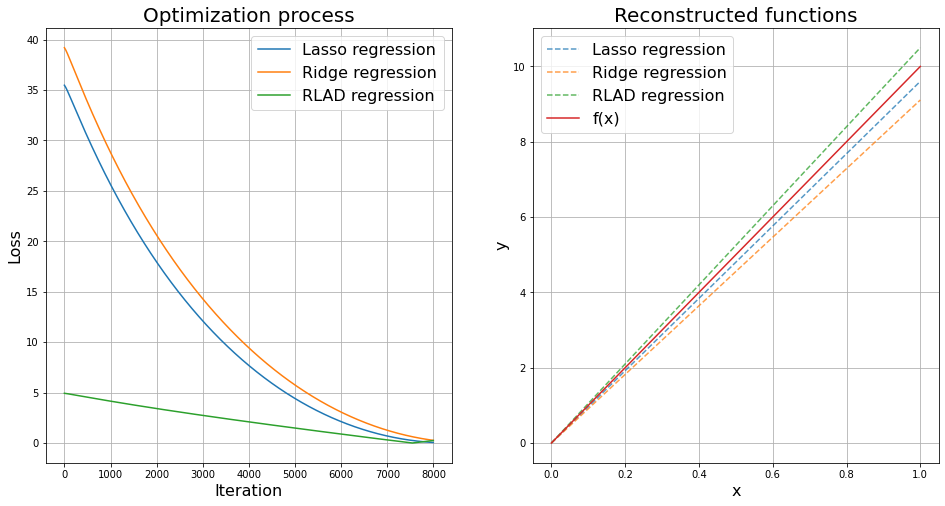
\includegraphics[width=\textwidth]{images/chapter2/reularization_impact.png}
	\caption{Comparison of different regularizations}
	\label{fig:regularizations}
\end{figure}